%!TEX root = ../report.tex

\section{Secure Channel}
A secure channel is a confidential, integrity protected and authenticated communication between two parties where messages are received in the correct order, no duplicates occur and if messages are missing we know which ones.\\

We will use the previously discussed cryptographic schemes to achieve this.
Despite knowing our modules to achieve most (confidentiality, authenticity) of the points from above, there are still some freedoms to put them together.\\
MAC-then-Encrypt ($Enc_{k-enc}(m,MAC_{k-int}(m))$) first authenticates the message and then encrypts the message as well as the MAC.
SSL uses this scheme, but many attacks on the protocol result from this.\\
MAC-and-Encrypt ($Enc_{k-enc}(m)$, $MAC_{k-int}(m)$) calculates the MAC and simply appends it to the encrypted message.
This approach is considered the weakest.\\
Encrypt-then-MAC ($Enc_{k-enc}(m)$, $MAC_{k-int}(Enc_{k-enc}(m))$) is the reversed approach compared to MAC-then-Encrypt.
It first encrypts the message and then calculates the MAC based on the encrypted message.
This approach is considered to be the most secure.\\
For loss and order detection it is possible to simply use a counter appended to the initial message.
It is necessary that it is at least authenticated.
Another note to be made here is that one has to make sure on implementation level that timing attacks are not possible.
Timing attacks look at how long certain operations take to get information about the system.

\subsection{Authenticated Encryption with Associated Data (AEAD)}
AEAD stands for a secure channel where data is sent that is first encrypted and then authenticated (Encrypt-then-MAC).
Additional to that, other data may be sent unencrypted but also authenticated.
Such data might be IVs, message counters, information necessary for message routing among others.\\
Special algorithms exist which need only one pass over the data to do this, most take two though.

\subsection{Offset Codebook Mode (OCB)}
OCB is such an one run encrypt and authenticate method.
\begin{figure}[H]
\centering
\begin{subfigure}{.5\textwidth}
  \centering
  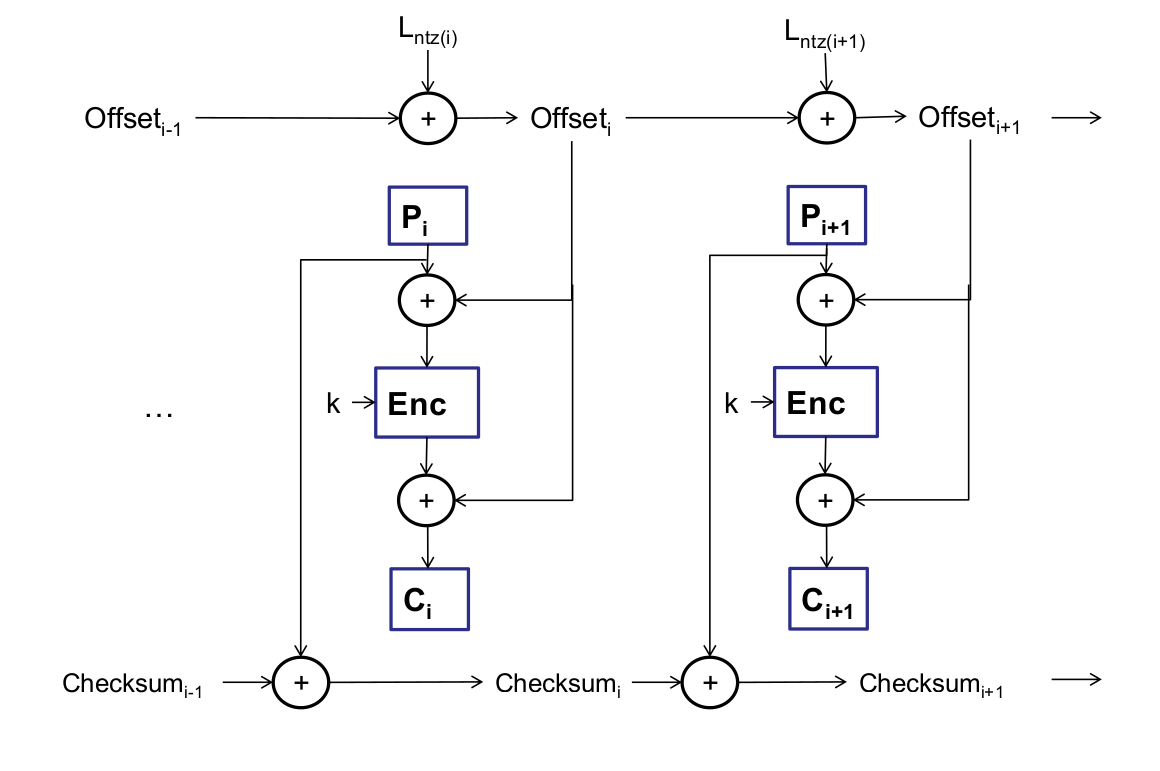
\includegraphics[width=\textwidth]{figures/ocb_encryption.png}
\end{subfigure}%
\begin{subfigure}{.5\textwidth}
  \centering
  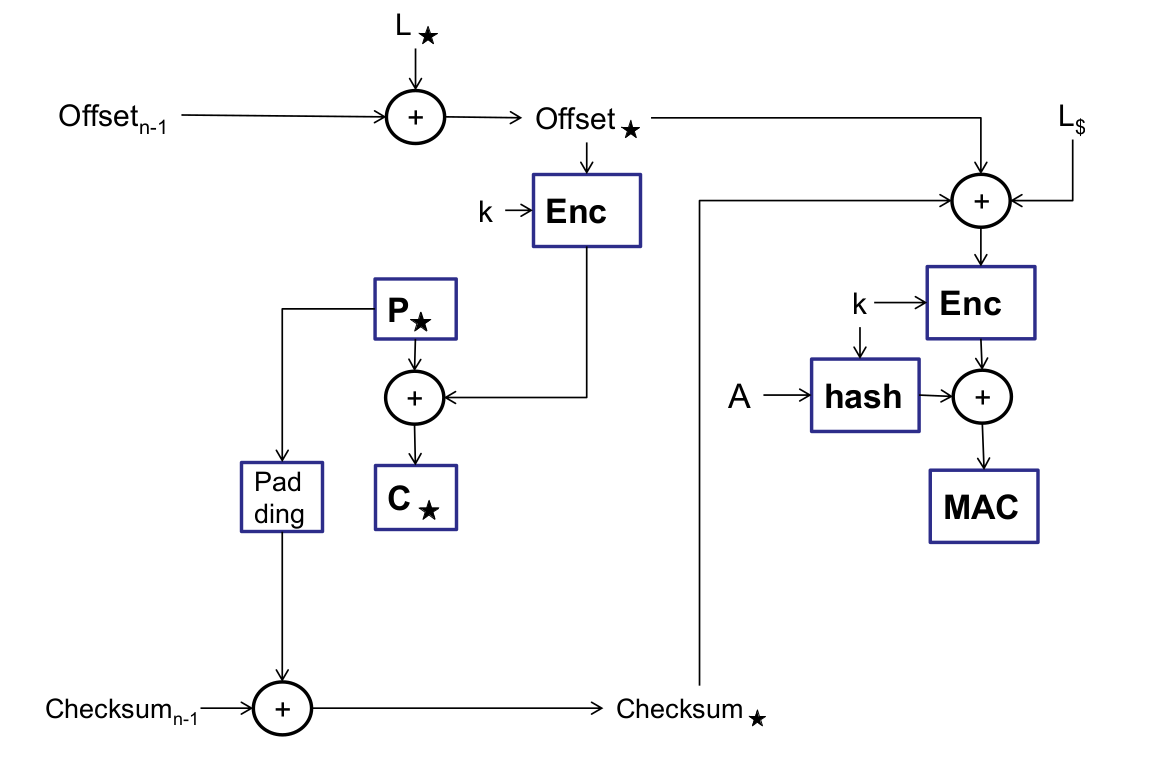
\includegraphics[width=\textwidth]{figures/ocb_mac.png}
\end{subfigure}
\caption{OCB}
\end{figure}
OCB works as described above with $L_* = Enc_k(0)$, $L_{\$} = double(L_*)$, $L_0 = double(L_{\$})$, $L_i = double(L_i) = double(L_{i-1})$ and $ntz = number~of~trailing~zeros$.
Most of the times only a view values for $L_i$ are used, but they can be precomputed and stored in a lookup table.
To note here is that OCB only needs one key for encryption and authentication but a fresh nonce for each run.

\subsection{Galois/Counter Mode (GCM)}
GCM is another one run approach to encrypt and authenticate.
It combines the concept of the counter mode for encryption with Galois Field Multiplication (based on $x^{128} + x^7 + x^2 + x + 1$) to compute the MAC on the ciphertext.
\begin{figure}[H]
  \centering
  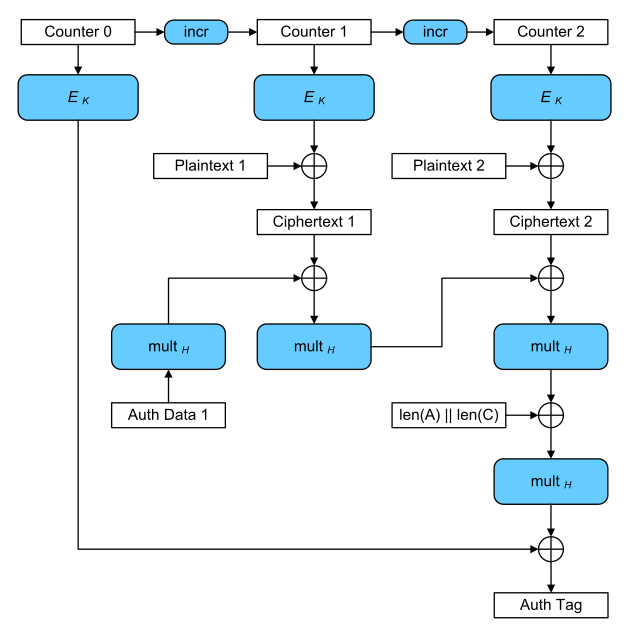
\includegraphics[width=.7\textwidth]{figures/gcm.png}
\end{figure}
GCM generates check values for $Auth~Data$, which is data that is not to be encrypted, by xoring and GF multiplication with $H = Enc(k,0)$.

\subsection{Attacks against a Secure Channel}
\subsubsection{Stream Ciphers}
Steam ciphers can be vulnerable to attacks if using the same IV multiple times.
Consider the following, where $KS(IV,k)$ is the keystream generated with key $k$ and initialization vector $IV$ and $C_i$ is the ciphertext calculated from the plaintext $P_i$ and the keystream
\begin{equation*}
  \begin{aligned}
    C_1 = P_1 \oplus KS(IV,k)\\
    C_2 = P_2 \oplus KS(IV,k).
  \end{aligned}
\end{equation*}
Xoring $C_1$ and $C_2$ results in
\begin{equation*}
  C_1 \oplus C_2 = P_1 \oplus KS(IV,k) \oplus P_2 \oplus KS(IV,k) = P_1 \oplus P_2\\
\end{equation*}
So the attacker can recover $P_1 \oplus P_2$ from $C_1$ and $C_2$ and if they know $P_1$ or $P_2$ they can recover the other.

\subsection{Padding Oracle Attack}
The padding oracle attack can reduce the attack time from $\mathcal{O}(N^L)$ to an average of $L \cdot \frac{N}{2}$ tries ($N$ is the size of the alphabet, $L$ the password/key length) under certain assumptions by decrypting ciphertexts bitwise.
These assumptions are:
\begin{enumerate}
  \item Attacker gets a ciphertext $C$ with $n$ blocks of length $N$
  \item Oracle that sends padding errors for wrong paddings and MAC errors if padding is correct.
    Can also be done with side channels like timings, \dots
  \item MAC-then-Encrypt is used (more precisely MAC-then-Encode-then-Encrypt, where first the MAC is calculated from the plaintext, then everything is padded to the block size and then encrypted)
  \item CBC is used
  \item PKCS7 padding scheme is used: 1 byte padding $\rightarrow$ 1, 2 byte padding $\rightarrow$ 2 2, \dots
\end{enumerate}

The attack starts decrypting the last byte of the last block of the massage $P_{n,N}$ by altering $C_{n-1,N}$ by xoring a value $\vartriangle$ to it $C_{n-1,N}' = C_{n-1,N} \oplus \vartriangle$.
$C_{n-1,N}'$ then is sent to the oracle.
If it responds with a padding error try again with a new $\vartriangle$ (max 256 tries, 1 byte!).
If it returns a MAC error though, we know that padding was fine and thus that $P_{n,N}' = 1$ (PKCS7 padding scheme!).
With that information we then can calculate $P_{n,N}$.
\begin{equation*}
  P_{n,N}' = P_{n,N} \oplus \vartriangle = 1 \rightarrow P_{n,N} = 1 \oplus \vartriangle
\end{equation*}

\begin{figure}[H]
  \centering
  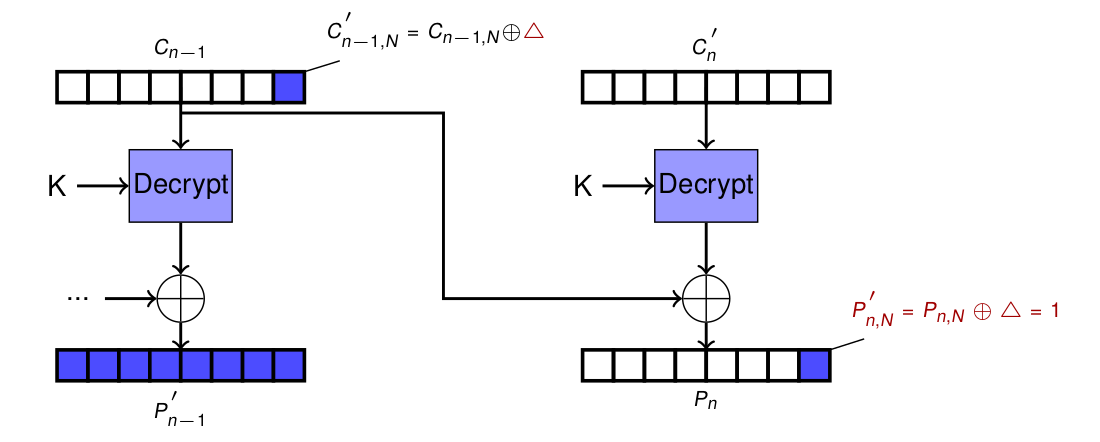
\includegraphics[width=.8\textwidth]{figures/padding_oracle_attack.png}
\end{figure}

Now we want to continue with $P_{n,N-1}$ for which we need a padding of length 2.
Since $P_{n,N}$ known, we can calculate $C_{n-1,N}'$ so that $P_{n,N}' = 2$ with
\begin{equation*}
  P_{n,N} \oplus C_{n-1,N}' = 2 \rightarrow C_{n-1,N}' = P_{n,N} \oplus 2
\end{equation*}
To find $P_{n,N-1}$ now, find a $C_{n-1,N-1}'$ that satisfies $C_{n-1,N}' \oplus P_{n,N-1} = 2$ with the same procedure as before.\\
To completely decrypt $C_n$ we have to repeat these steps until all bytes of the block are decrypted.
To decrypt $C_{n-1}$ we can just simply cut off $C_n$ and do the same again.
For $C_1$ the IV is used as ciphertext for the attack modifications.
